Figure \ref{fig:CSA_Lookup_diff_texts} shows comparative characteristics of substring lookup
for different textual data.

\begin{figure}[h!]
    \centering
    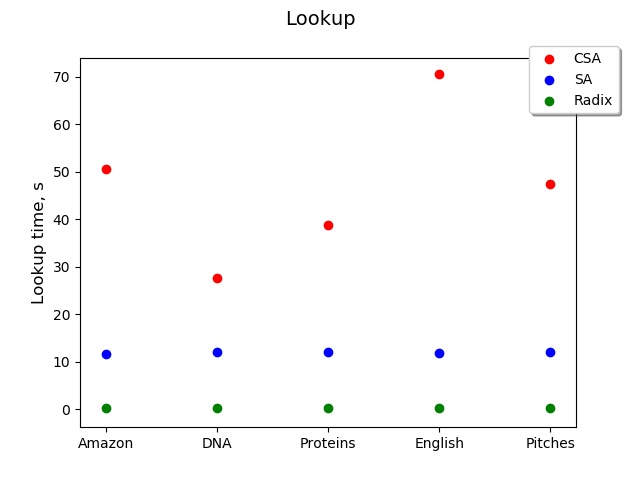
\includegraphics[width=12cm]{lookup_diff_texts}
    \caption{Substring lookup in CSA}
    \label{fig:CSA_Lookup_diff_texts}
\end{figure}

Let us consider relative compression of the CSA in respect to a suffix array.
Mean ratio of memory used for CSA to memory used for suffix array is calculated
depending on the size of the initial text. Figure \ref{fig:CSA_compression_ratio_amazon} shows
a reduction of the ratio, that is compression coefficient increase.
Remarkably, for small sizes of the initial text CSA takes more space than suffix array.
It is explained by the usage of additional data structures descibed at the previous pages.
At the CSA construction they consume memory comparable by the order to the index size
in a succinct representation. For large texts CSA becomes more effective in comparison to
classic suffix array.

\begin{figure}[h!]
    \centering
    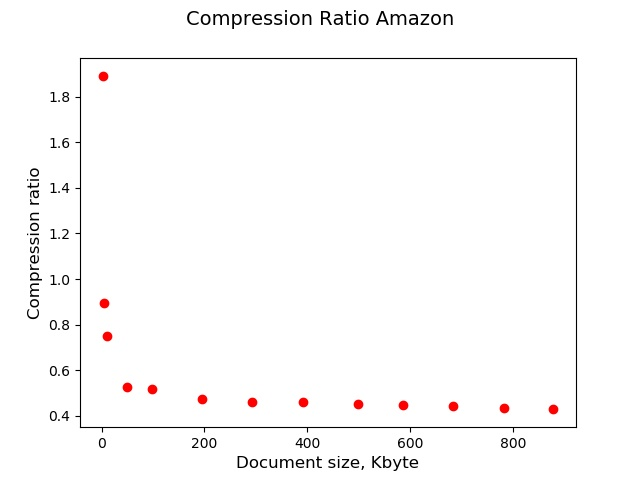
\includegraphics[width=12cm]{compression_ratio_amazon}
    \caption{Compression ratio of CSA to SA}
    \label{fig:CSA_compression_ratio_amazon}
\end{figure}

Relative compression CSA/SA for different texts is shown at the figure \ref{fig:CSA_compression_ratio_dif_texts}.
It is possible to explicitly notice the dependency between a succinct index size from the alphabet size,
that can not be said about suffix array and radix tree.

\begin{figure}[h!]
    \centering
    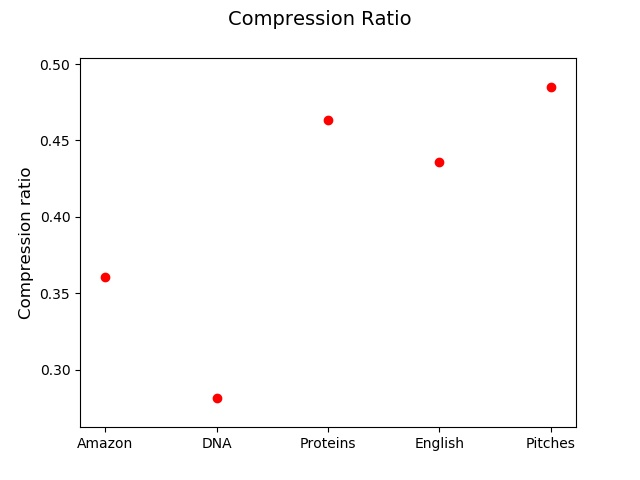
\includegraphics[width=12cm]{compression_ratio_dif_texts}
    \caption{Compression ratio of CSA to SA}
    \label{fig:CSA_compression_ratio_dif_texts}
\end{figure}
